\documentclass[a4paper,12pt]{article}
\usepackage{indentfirst}
\usepackage[T1]{fontenc}
\usepackage{graphicx}
\usepackage{booktabs}
\usepackage{array}
\usepackage{tabularx}
\usepackage{float}
\usepackage{caption}
\usepackage{subcaption}
\graphicspath{{../Imagens/}{Imagens/}}
\renewcommand{\figurename}{Figura}
\renewcommand{\tablename}{Tabela}
\captionsetup{
  justification=raggedright,
  singlelinecheck=false,
  labelsep=endash,
  font=small,
  labelfont=bf,
  skip=6pt
}
\captionsetup[figure]{position=above}
\captionsetup[table]{position=above}
\newfloat{quadro}{htbp}{loq}
\floatname{quadro}{Quadro}
\captionsetup[quadro]{position=above}
\newcommand{\fonteelemento}[1]{%
  \par\smallskip
  {\footnotesize\raggedright Fonte: #1.\par}%
}

\begin{document}

\section{Materiais e M\'etodos}


Este cap\'itulo descreve os recursos empregados na constru\c{c}\~ao do prot\'otipo, o m\'etodo adotado para desenvolver a plataforma e os procedimentos definidos para sua avalia\c{c}\~ao. A descri\c{c}\~ao da implementa\c{c}\~ao interna dos servi\c{c}os, drivers e m\'odulos \'e apresentada no cap\'itulo de Desenvolvimento, enquanto os valores medidos e sua interpreta\c{c}\~ao pertencem ao cap\'itulo de Resultados e Discuss\~ao.


Os procedimentos de ensaio foram formulados para permitir repeti\c{c}\~ao sob condi\c{c}\~oes declaradas. O firmware integrado, o caderno de ensaios, os arquivos de dados, os scripts de tratamento e as imagens correspondentes foram usados para distinguir procedimentos executados de pilotos, observa\c{c}\~oes qualitativas e atividades retiradas do escopo temporal desta vers\~ao. Nenhum resultado \'e antecipado neste cap\'itulo.


\subsection{Materiais}


\subsubsection{Unidade de processamento}


A unidade de processamento utilizada foi a placa Seeed Studio XIAO ESP32-C6, baseada no sistema em chip ESP32-C6. O processador principal emprega arquitetura RISC-V de 32 bits e opera a at\'e 160 MHz. O dispositivo disp\~oe de 512 KiB de SRAM de alto desempenho e a placa cont\'em 4 MiB de mem\'oria \emph{flash}. Seu formato de 21 $\times$ 17,8 mm permite o encaixe na placa de expans\~ao circular utilizada no prot\'otipo (SEEED STUDIO, 2024).


A escolha considerou a compatibilidade mec\^anica com o Round Display, a disponibilidade de controladores para I$^2$C, SPI, RMT e GPIO, os recursos necess\'arios \`a interface gr\'afica e o suporte oficial do ESP-IDF. As interfaces sem fio presentes no ESP32-C6 n\~ao constitu\'iram requisito da vers\~ao avaliada e n\~ao foram utilizadas como justificativa de resultados de conectividade ou consumo.


\subsubsection{Round Display}


A interface f\'isica foi constru\'ida sobre o Seeed Studio Round Display for XIAO, uma placa circular de 39 mm com display sens\'ivel ao toque de 1,28 polegada, resolu\c{c}\~ao de 240 $\times$ 240 pixels e profundidade de 16 bits. A placa tamb\'em cont\'em circuito de carregamento para bateria, conector para bateria, slot para cart\~ao microSD e um RTC PCF8563 (SEEED STUDIO, [s.d.]).


O painel \'e controlado pelo GC9A01A e recebe comandos e pixels RGB565 pelo perif\'erico SPI2. No prot\'otipo, a interface opera a 40 MHz e utiliza somente transmiss\~ao para o display. O toque capacitivo do exemplar utilizado \'e controlado pelo CHSC6X, identificado no endere\c{c}o I$^2$C 0x2E. Essa identifica\c{c}\~ao decorre do hardware efetivamente recebido e difere do controlador indicado em parte da documenta\c{c}\~ao hist\'orica da placa.


O PCF8563, no endere\c{c}o I$^2$C 0x51, mant\'em segundos, minutos, horas e calend\'ario. A bateria de reserva instalada no Round Display permite conservar essas informa\c{c}\~oes quando a alimenta\c{c}\~ao principal \'e removida. O backlight permaneceu ligado durante a opera\c{c}\~ao porque seu controle por software n\~ao ficou dispon\'ivel na combina\c{c}\~ao de revis\~ao de placa e XIAO ESP32-C6 utilizada.


\subsubsection{Sensores}


\paragraph{MAX30102}


O MAX30102 \'e um sensor \'optico reflexivo que integra emissores vermelho e infravermelho, fotodetector, conversor de 18 bits, rejei\c{c}\~ao de luz ambiente e FIFO com 32 posi\c{c}\~oes. O componente comunica-se por I$^2$C no endere\c{c}o 0x57 e permite configurar corrente dos emissores, largura dos pulsos, taxa de amostragem e faixa do conversor (ANALOG DEVICES, 2018).


No prot\'otipo, o sensor foi empregado para adquirir os canais de PPG utilizados na estimativa de frequ\^encia card\'iaca e de SpO$_2$. A placa de conex\~ao utilizada integra a alimenta\c{c}\~ao exigida pelo componente. Como os resultados n\~ao possuem valida\c{c}\~ao cl\'inica, o m\'odulo foi tratado como demonstrador de aquisi\c{c}\~ao e processamento de sinais fisiol\'ogicos.


\paragraph{DS18B20}


O DS18B20 \'e um sensor digital de temperatura com interface 1-Wire, resolu\c{c}\~ao configur\'avel entre 9 e 12 bits e verifica\c{c}\~ao CRC dos dados. Foi utilizado com alimenta\c{c}\~ao externa de 3,3 V, resolu\c{c}\~ao de 11 bits e resistor de \emph{pull-up} de 4,7 k$\Omega$ entre a linha de dados e a alimenta\c{c}\~ao. A comunica\c{c}\~ao foi realizada no GPIO20 por meio do perif\'erico RMT e dos componentes oficiais \texttt{onewire\_bus} e \texttt{ds18b20} (ANALOG DEVICES, 2019).


O sensor foi destinado \`a observa\c{c}\~ao de temperatura ambiente. Sua posi\c{c}\~ao na montagem provis\'oria, a aus\^encia de encapsulamento final e a influ\^encia t\'ermica do pr\'oprio prot\'otipo devem ser registradas em cada ensaio, pois uma leitura no dispositivo n\~ao representa automaticamente a temperatura corporal.


\paragraph{LTR390}


O LTR390 integra um canal para luz ambiente e outro para radia\c{c}\~ao ultravioleta, selecionados de forma alternada, e fornece os resultados por I$^2$C no endere\c{c}o 0x53. Ganho e tempo de integra\c{c}\~ao configur\'aveis determinam a resolu\c{c}\~ao e o limite de satura\c{c}\~ao. A convers\~ao das contagens depende da configura\c{c}\~ao aplicada e das rela\c{c}\~oes fornecidas pelo fabricante (LITE-ON TECHNOLOGY, 2024).


O mesmo componente foi empregado para estimar ilumin\^ancia e UVI. Como os canais n\~ao s\~ao convertidos simultaneamente, o m\'etodo de opera\c{c}\~ao alterna o modo conforme a fun\c{c}\~ao ativa e descarta as primeiras amostras ap\'os a mudan\c{c}a para permitir a estabiliza\c{c}\~ao. A estimativa de UVI do prot\'otipo n\~ao foi equiparada a uma medi\c{c}\~ao meteorol\'ogica de refer\^encia.


\paragraph{MPU-9250 e AK8963}


O m\'odulo inercial empregado foi baseado no MPU-9250, que re\'une aceler\^ometro e girosc\'opio triaxiais e permite acesso ao magnet\^ometro AK8963. O MPU-9250 foi ligado ao barramento I$^2$C no endere\c{c}o 0x68; o AK8963 foi acessado no endere\c{c}o 0x0C por meio do modo \emph{bypass} do MPU-9250 (TDK INVENSENSE, 2016).


As acelera\c{c}\~oes foram utilizadas pelo ped\^ometro implementado em software. As medidas magn\'eticas foram utilizadas para a b\'ussola ap\'os corre\c{c}\~ao de deslocamento e escala obtida por calibra\c{c}\~ao executada no pr\'oprio dispositivo. Os par\^ametros de calibra\c{c}\~ao foram armazenados em mem\'oria n\~ao vol\'atil. O c\'alculo de \emph{heading} n\~ao inclui compensa\c{c}\~ao de inclina\c{c}\~ao e pressup\~oe que o dispositivo esteja aproximadamente nivelado.


\subsubsection{Instrumentos de bancada}

Foram empregados um mult\'imetro digital para medir tens\~ao e corrente, um ox\'imetro de dedo ECH de modelo n\~ao identificado para compara\c{c}\~ao funcional de frequ\^encia card\'iaca e SpO$_2$, um termo-higr\^ometro MFL modelo Embutir para compara\c{c}\~ao de temperatura e uma b\'ussola magn\'etica Norvix DC45-2 para compara\c{c}\~ao de \emph{heading}. Um Amazfit Active 2 foi usado como corrobora\c{c}\~ao no ensaio de PPG e como comparador secund\'ario no ensaio do ped\^ometro. Uma lanterna comum e uma lanterna UV gen\'erica foram utilizadas somente como est\'imulos funcionais dos canais de ilumin\^ancia e ultravioleta do LTR390.

Os instrumentos de consumo n\~ao possu\'iam certificado de calibra\c{c}\~ao dispon\'ivel. Consequentemente, as compara\c{c}\~oes foram classificadas como testes funcionais ou verifica\c{c}\~oes de plausibilidade, e n\~ao como valida\c{c}\~oes metrol\'ogicas ou cl\'inicas. As fotografias do ox\'imetro e do termo-higr\^ometro correspondem aos aparelhos efetivamente empregados.


\subsubsection{Ferramentas de software}


O firmware foi desenvolvido em C com ESP-IDF 5.5.1. O FreeRTOS fornecido pelo ambiente foi utilizado em configura\c{c}\~ao de n\'ucleo \'unico, e a interface gr\'afica foi constru\'ida com LVGL v8. O SquareLine Studio 1.6.0 foi empregado somente na cria\c{c}\~ao da base visual da tela principal, aproximando-a do desenho pretendido. Como os recursos gr\'aficos exportados ocupavam parcela relevante da mem\'oria flash, as demais telas foram implementadas diretamente com a API do LVGL. A compila\c{c}\~ao e a an\'alise do tamanho da aplica\c{c}\~ao utilizaram as ferramentas do ESP-IDF. O monitor serial e os n\'iveis de log foram empregados no diagn\'ostico de inicializa\c{c}\~ao, comunica\c{c}\~ao e tarefas.


Foram usados os componentes LVGL 8.4.0, \texttt{esp\_lcd\_gc9a01} 2.0.4, \texttt{esp\_lcd\_touch} 1.2.1, \texttt{esp\_lvgl\_port} 2.8.0-1, \texttt{onewire\_bus} 1.1.1 e \texttt{ds18b20} 0.1.2, conforme o arquivo \texttt{dependencies.lock}. Drivers pr\'oprios foram adotados para MAX30102, LTR390, MPU-9250/AK8963, PCF8563 e CHSC6X.


\subsubsection{Montagem e mapa de liga\c{c}\~oes}


A integra\c{c}\~ao f\'isica foi realizada em uma placa prot\'otipo autoral, acompanhada de inv\'olucro fabricado por impress\~ao 3D. O XIAO ESP32-C6 permaneceu encaixado no Round Display, e os sensores externos foram distribu\'idos na placa conforme o esquema e o leiaute documentados. O barramento I$^2$C foi compartilhado pelos sensores, pelo toque e pelo RTC, operando a 100 kHz em SDA GPIO22 e SCL GPIO23. A Figura~\ref{fig:placa-prototipo} registra a placa em funcionamento, enquanto a Figura~\ref{fig:pcb-render} apresenta as duas faces previstas no projeto.


\begin{figure}[H]
\centering
\caption{Placa prot\'otipo com display e m\'odulos durante a opera\c{c}\~ao}
\label{fig:placa-prototipo}
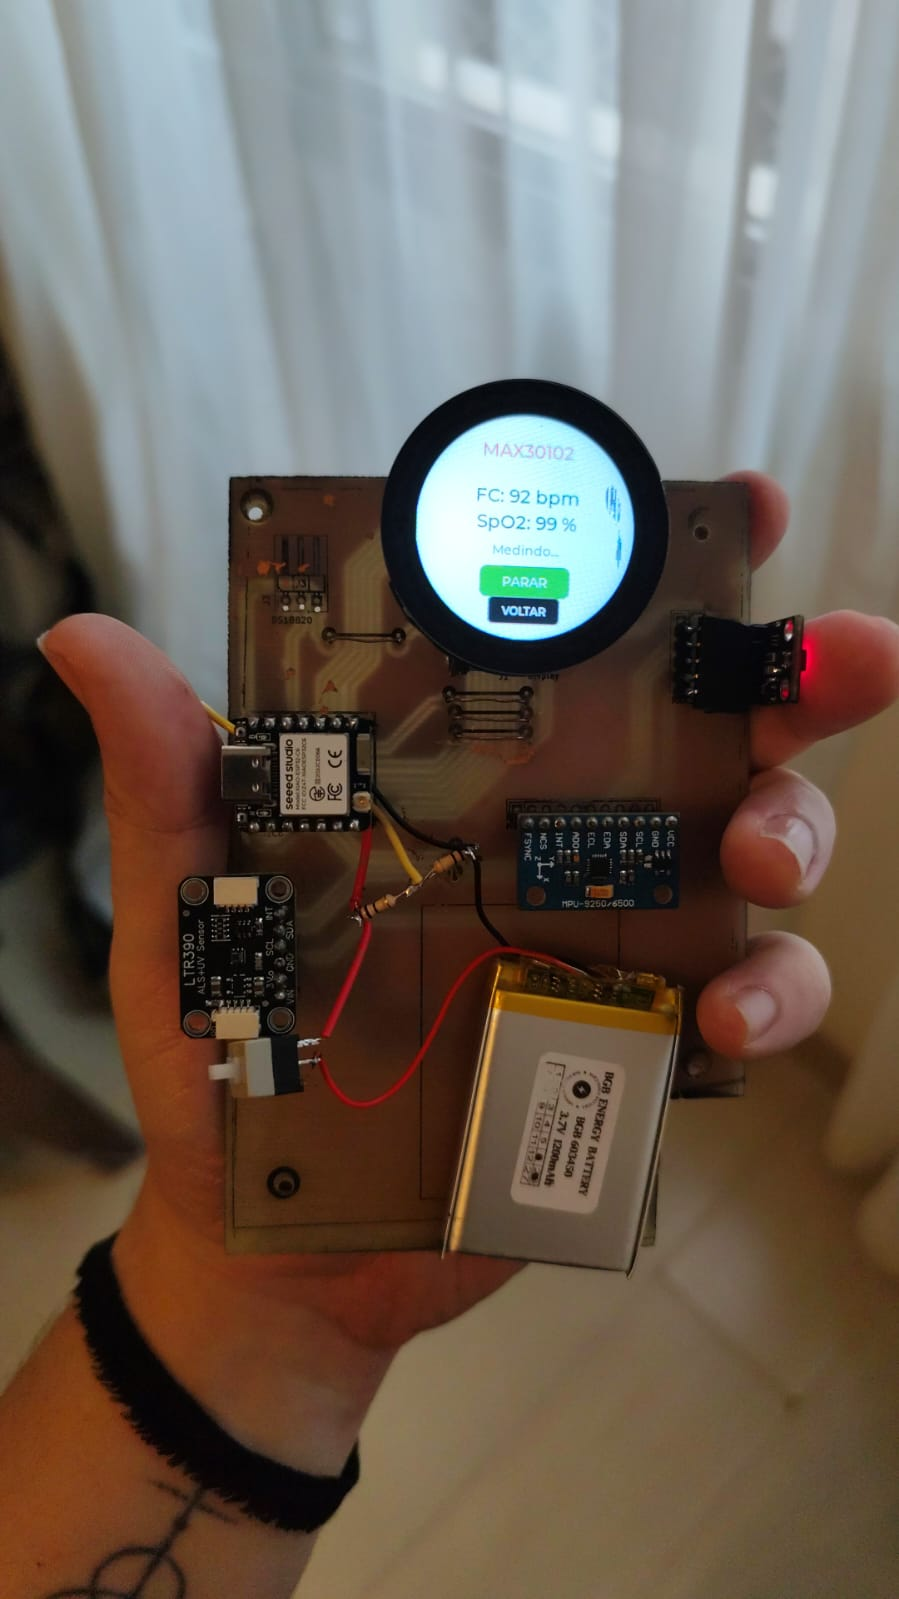
\includegraphics[width=0.48\textwidth]{PCB/Prototipo.jpeg}
\begin{minipage}{0.48\textwidth}
\fonteelemento{Acervo do autor}
\end{minipage}
\end{figure}


\begin{figure}[H]
\centering
\caption{Renderiza\c{c}\~oes das faces da placa desenvolvida}
\label{fig:pcb-render}
\begin{subfigure}[t]{0.44\textwidth}
\centering
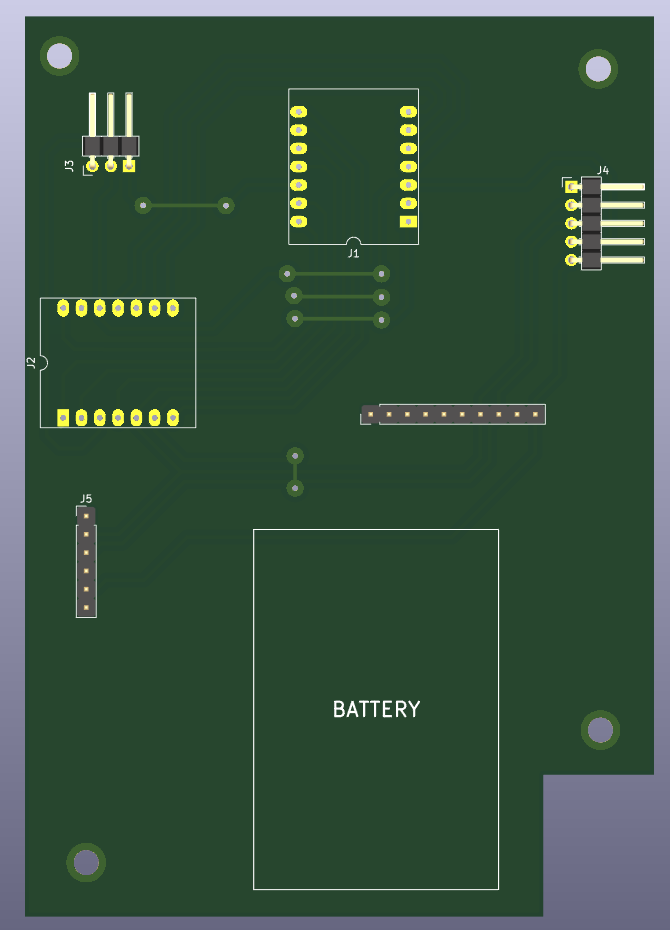
\includegraphics[width=\linewidth]{PCB/3dtoplayer.png}
\caption{Face superior}
\end{subfigure}
\hfill
\begin{subfigure}[t]{0.44\textwidth}
\centering
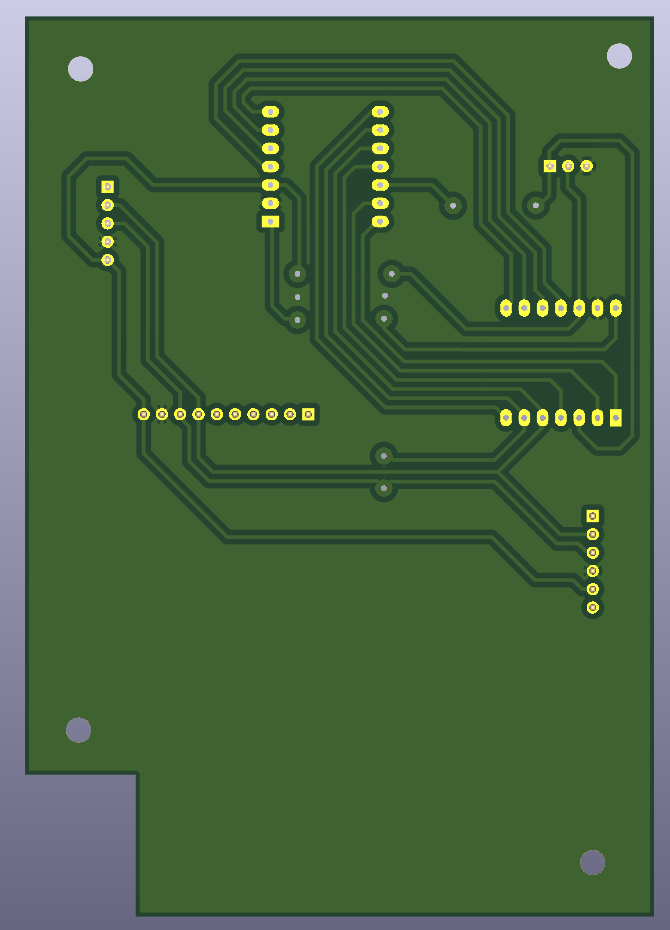
\includegraphics[width=\linewidth]{PCB/3dbottomlayer.png}
\caption{Face inferior}
\end{subfigure}
\begin{minipage}{0.92\textwidth}
\fonteelemento{Elaborado pelo autor a partir do projeto da placa}
\end{minipage}
\end{figure}


O Quadro~\ref{qua:mapa-interfaces} consolida as interfaces e conex\~oes confirmadas no firmware integrado.


\begin{quadro}[H]
\centering
\caption{Mapa consolidado de interfaces e liga\c{c}\~oes}
\label{qua:mapa-interfaces}
\small
\renewcommand{\arraystretch}{1.12}
\begin{tabularx}{\textwidth}{|>{\raggedright\arraybackslash}p{0.20\textwidth}|>{\raggedright\arraybackslash}p{0.19\textwidth}|>{\raggedright\arraybackslash}X|>{\raggedright\arraybackslash}p{0.25\textwidth}|}
\hline
\textbf{Elemento} & \textbf{Interface} & \textbf{Endere\c{c}o ou sinais} & \textbf{Conex\~ao no ESP32-C6} \\
\hline
GC9A01A & SPI2, 40 MHz & SCLK, MOSI, CS e D/C & GPIO19, GPIO18, GPIO1 e GPIO21 \\
\hline
CHSC6X & I$^2$C & 0x2E; interrup\c{c}\~ao ativa & SDA GPIO22, SCL GPIO23 e INT GPIO17 \\
\hline
PCF8563 & I$^2$C & 0x51 & SDA GPIO22 e SCL GPIO23 \\
\hline
LTR390 & I$^2$C & 0x53 & SDA GPIO22 e SCL GPIO23 \\
\hline
MAX30102 & I$^2$C & 0x57 & SDA GPIO22 e SCL GPIO23 \\
\hline
MPU-9250 & I$^2$C & 0x68 & SDA GPIO22 e SCL GPIO23 \\
\hline
AK8963 & I$^2$C via \emph{bypass} & 0x0C & barramento compartilhado pelo MPU-9250 \\
\hline
DS18B20 & 1-Wire por RMT & DQ com \emph{pull-up} de 4,7 k$\Omega$ & GPIO20 \\
\hline
Bateria & ADC & divisor resistivo 1:2 & GPIO0 \\
\hline
\end{tabularx}
\fonteelemento{Elaborado pelo autor a partir do firmware integrado e do projeto da placa}
\end{quadro}


A representa\c{c}\~ao gr\'afica correspondente \'e mostrada na Figura~\ref{fig:mapa-ligacoes}.


\begin{figure}[H]
\centering
\caption{Mapa de liga\c{c}\~oes da montagem final}
\label{fig:mapa-ligacoes}
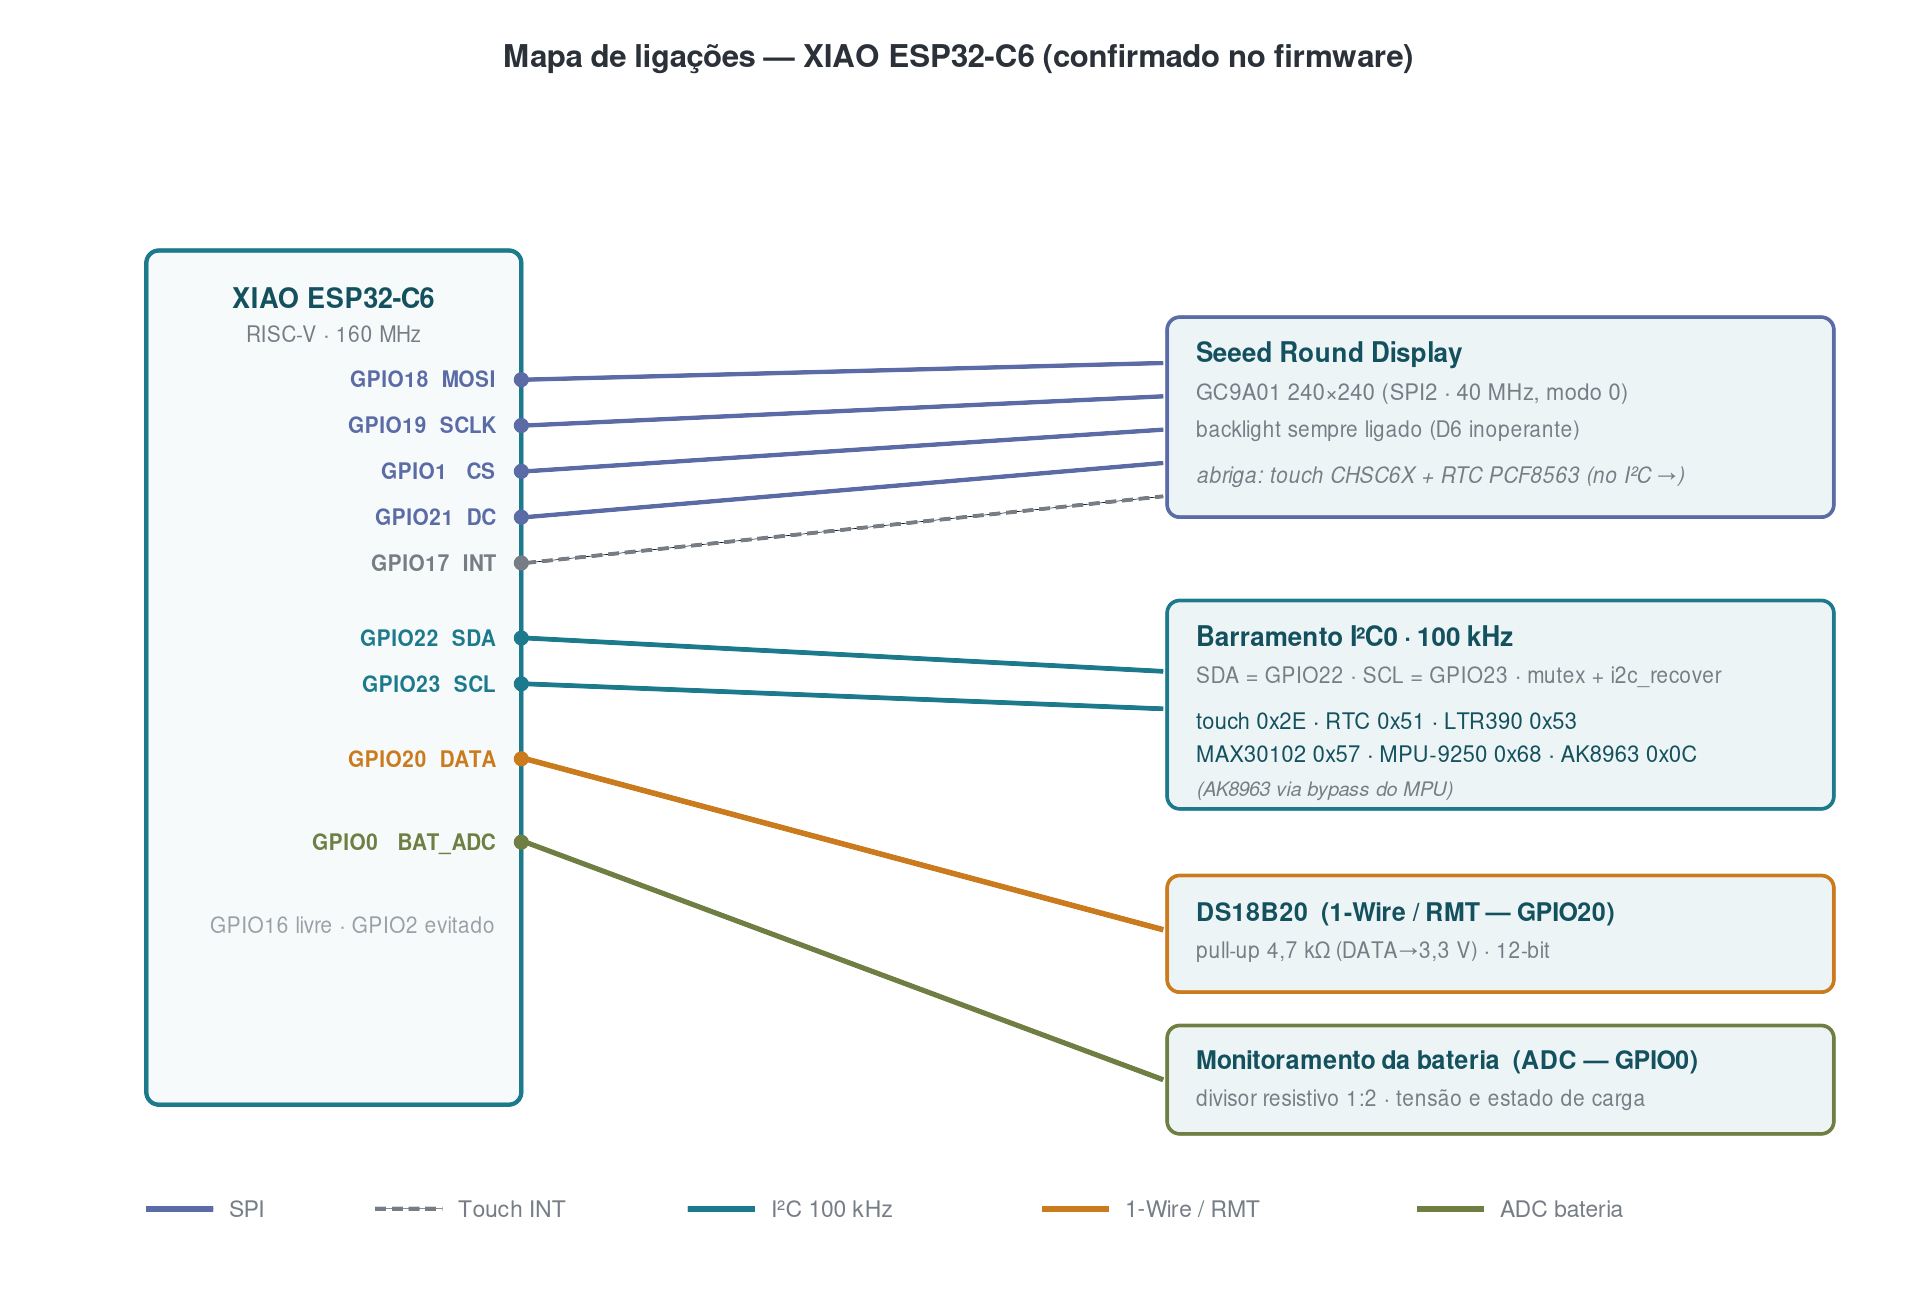
\includegraphics[width=0.95\textwidth]{Diagramas/sistema/mapa_ligacoes.png}
\fonteelemento{Elaborado pelo autor a partir do firmware integrado e do projeto da placa}
\end{figure}


Todos os m\'odulos compartilharam a refer\^encia de terra e foram alimentados em n\'iveis compat\'iveis com suas placas de conex\~ao. O esquema, o leiaute e a fotografia foram preservados como registros complementares da montagem utilizada.


\subsection{Metodologia de desenvolvimento}


\subsubsection{Levantamento de requisitos}


Os requisitos foram derivados do problema de integrar fun\c{c}\~oes independentes em uma plataforma vest\'ivel com recursos compartilhados. Foram definidos como requisitos funcionais a apresenta\c{c}\~ao de hora e data, a navega\c{c}\~ao por toque, a aquisi\c{c}\~ao dos sensores biom\'etricos, ambientais e inerciais e a apresenta\c{c}\~ao de suas informa\c{c}\~oes em telas pr\'oprias.


Os requisitos arquiteturais estabeleceram que cada fun\c{c}\~ao sensorial deveria ser encapsulada em um m\'odulo, que novos m\'odulos pudessem ser inclu\'idos com altera\c{c}\~oes localizadas e que a aus\^encia de um sensor n\~ao impedisse a continuidade das fun\c{c}\~oes independentes. O acesso concorrente ao I$^2$C deveria ser serializado, e erros de comunica\c{c}\~ao n\~ao poderiam provocar espera indefinida nem interromper deliberadamente toda a inicializa\c{c}\~ao.


Como restri\c{c}\~oes foram considerados o processamento em n\'ucleo \'unico, a mem\'oria dispon\'ivel, a parti\c{c}\~ao de aplica\c{c}\~ao de aproximadamente 1 MiB, o display circular de 240 $\times$ 240 pixels, a coexist\^encia de dispositivos no mesmo I$^2$C e a indisponibilidade de controle do backlight. Gerenciamento avan\c{c}ado de energia, valida\c{c}\~ao cl\'inica, persist\^encia do ped\^ometro, conectividade sem fio e compensa\c{c}\~ao de inclina\c{c}\~ao da b\'ussola foram exclu\'idos da vers\~ao avaliada.


\subsubsection{Crit\'erios de sele\c{c}\~ao de componentes}


A sele\c{c}\~ao partiu da necessidade de representar transportes e classes de sensoriamento diferentes em uma \'unica plataforma. O XIAO ESP32-C6 e o Round Display formaram a base pela compatibilidade mec\^anica, pelas dimens\~oes e pela disponibilidade dos perif\'ericos necess\'arios. O display circular, o toque e o RTC permitiram construir a interface demonstradora sem uma placa gr\'afica adicional.


O MAX30102 foi escolhido por integrar aquisi\c{c}\~ao PPG reflexiva em dois comprimentos de onda. O DS18B20 acrescentou um sensor digital em interface 1-Wire independente do I$^2$C. O LTR390 reuniu luz ambiente e ultravioleta em um \'unico dispositivo. O MPU-9250, com o AK8963, permitiu utilizar a mesma unidade para pedometria e orienta\c{c}\~ao magn\'etica.


Disponibilidade, documenta\c{c}\~ao e exist\^encia pr\'evia dos componentes tamb\'em influenciaram a escolha. N\~ao foi realizada compara\c{c}\~ao experimental sistem\'atica com microcontroladores ou sensores alternativos; portanto, a sele\c{c}\~ao representa uma decis\~ao de projeto segundo os requisitos e recursos dispon\'iveis, e n\~ao a demonstra\c{c}\~ao de superioridade desses componentes.


\subsubsection{Defini\c{c}\~ao da arquitetura}


A arquitetura foi definida pela separa\c{c}\~ao entre n\'ucleo da aplica\c{c}\~ao, servi\c{c}os compartilhados, drivers de hardware e m\'odulos funcionais. Cada m\'odulo foi concebido como uma unidade autocontida com opera\c{c}\~oes de inicializa\c{c}\~ao, cria\c{c}\~ao de tela e exibi\c{c}\~ao de tela. O n\'ucleo registra essas opera\c{c}\~oes e coordena a navega\c{c}\~ao sem incorporar o processamento espec\'ifico de cada sensor.


As aquisi\c{c}\~oes peri\'odicas foram atribu\'idas a tarefas independentes. Quando uma aquisi\c{c}\~ao s\'o era necess\'aria para atualizar uma tela, sua execu\c{c}\~ao foi condicionada \`a tela ativa. Servi\c{c}os comuns concentraram o acesso \`a interface gr\'afica, ao barramento I$^2$C e \`a persist\^encia em NVS. O contrato e as depend\^encias concretas da implementa\c{c}\~ao s\~ao apresentados no cap\'itulo de Desenvolvimento.


A extensibilidade foi considerada durante a defini\c{c}\~ao dos pontos de registro e das interfaces. A inicializa\c{c}\~ao n\~ao fatal e a recupera\c{c}\~ao do I$^2$C tamb\'em foram incorporadas \`a arquitetura. A avalia\c{c}\~ao desta vers\~ao combinou estudo retrospectivo de integra\c{c}\~ao, an\'alise est\'atica das depend\^encias e ensaios qualitativos com remo\c{c}\~ao individual e combinada dos sensores; a efic\'acia din\^amica da recupera\c{c}\~ao do barramento permaneceu fora do escopo experimental.


\subsubsection{Desenvolvimento incremental}


O desenvolvimento foi conduzido em etapas. Cada componente foi inicialmente estudado a partir da folha de dados e exercitado isoladamente, com inspe\c{c}\~ao de identifica\c{c}\~ao, configura\c{c}\~ao e dados brutos. Em seguida, sua aquisi\c{c}\~ao e seu processamento foram separados do c\'odigo de apresenta\c{c}\~ao, e o m\'odulo foi incorporado ao contrato comum da plataforma.


A integra\c{c}\~ao ocorreu progressivamente para permitir localizar conflitos de endere\c{c}amento, temporiza\c{c}\~ao, alimenta\c{c}\~ao e mem\'oria. Ap\'os cada inclus\~ao, foram verificados inicializa\c{c}\~ao, resposta da interface, logs de erro e continuidade das fun\c{c}\~oes j\'a existentes. Problemas observados durante essa evolu\c{c}\~ao orientaram a redu\c{c}\~ao do I$^2$C para 100 kHz, a serializa\c{c}\~ao por mutex, a recupera\c{c}\~ao p\'os-NACK, o aumento do pool do LVGL e o condicionamento das aquisi\c{c}\~oes pela tela ativa. A Figura~\ref{fig:metodo-incremental} sintetiza o ciclo aplicado.


\begin{figure}[H]
\centering
\caption{M\'etodo incremental de desenvolvimento e integra\c{c}\~ao}
\label{fig:metodo-incremental}
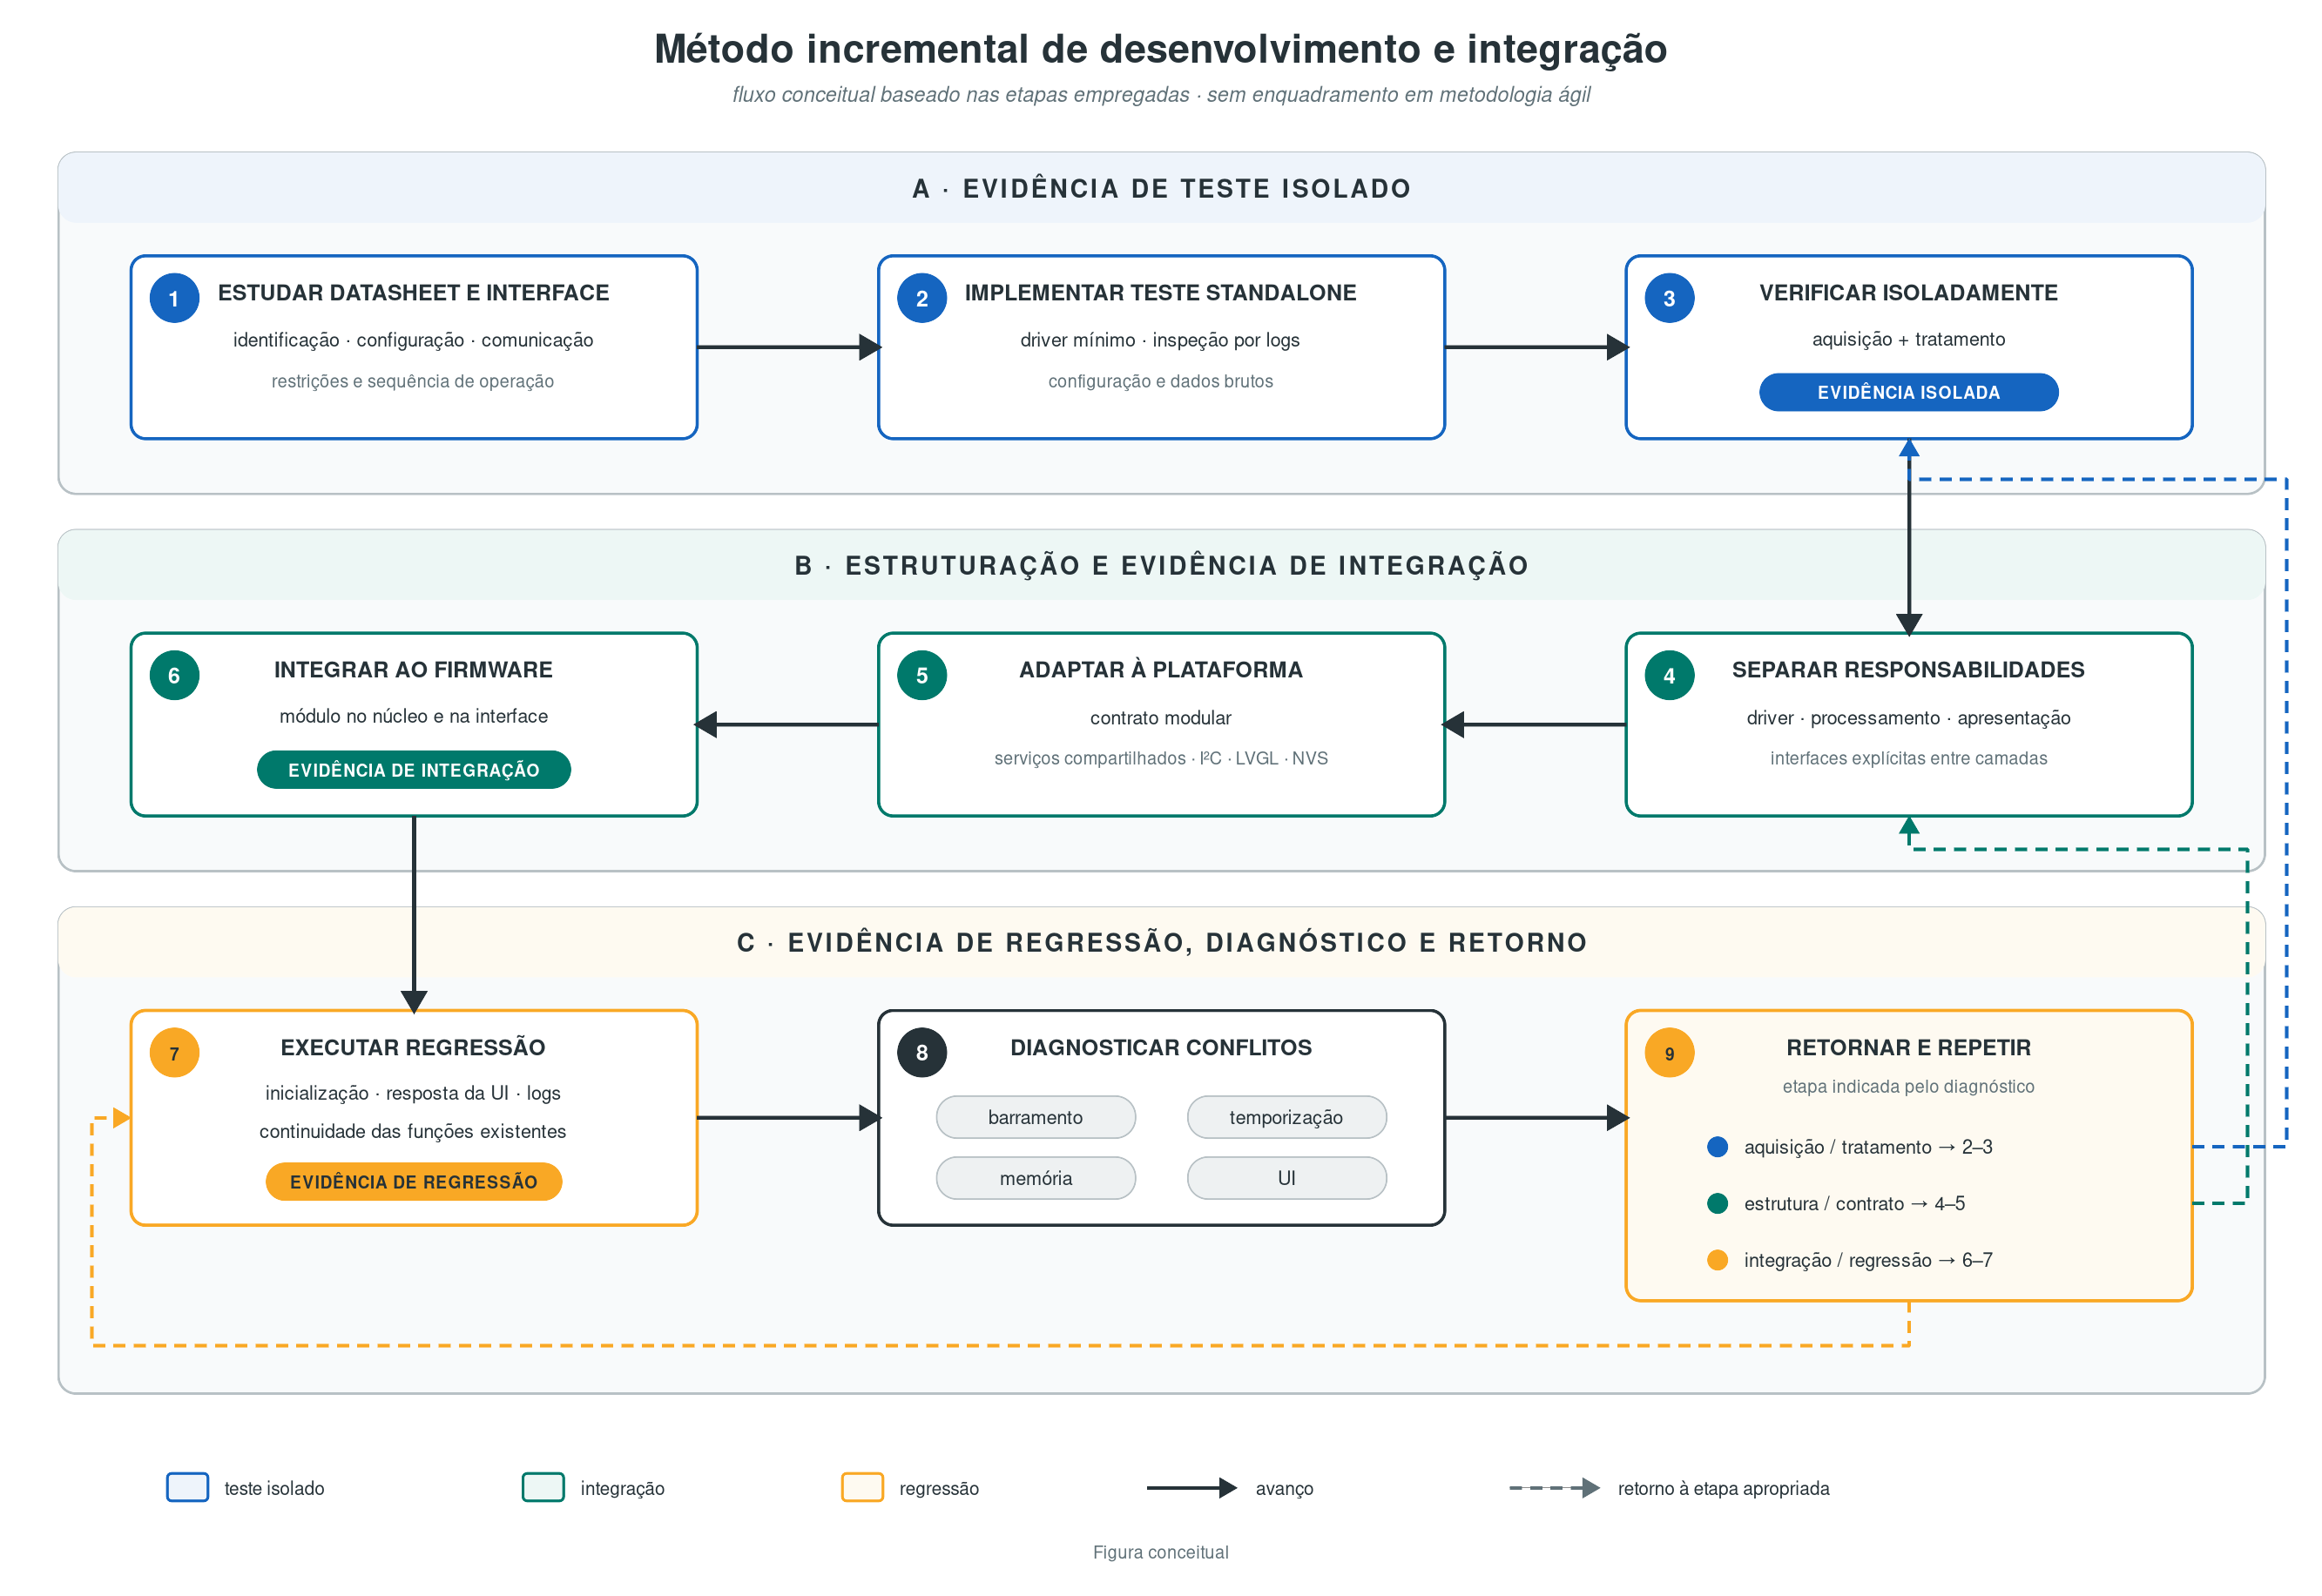
\includegraphics[width=0.96\textwidth]{Diagramas/teoricas/metodo_incremental.png}
\fonteelemento{Elaborado pelo autor a partir do procedimento empregado no projeto}
\end{figure}


As corre\c{c}\~oes realizadas durante o desenvolvimento n\~ao constituem, isoladamente, ensaios finais. Para que uma observa\c{c}\~ao de depura\c{c}\~ao seja apresentada como resultado, ela dever\'a ser repetida segundo um dos procedimentos definidos neste cap\'itulo e acompanhada de vers\~ao do firmware, condi\c{c}\~oes, dados e crit\'erio de interpreta\c{c}\~ao.


\subsubsection{Crit\'erios para drivers pr\'oprios e componentes oficiais}


Um componente oficial foi preferido quando oferecia compatibilidade com o ESP-IDF 5.5.1, utilizava as APIs atuais, apresentava manuten\c{c}\~ao e encapsulava adequadamente o perif\'erico sem impedir a integra\c{c}\~ao arquitetural. Esse crit\'erio foi aplicado ao controlador do display, \`a porta do LVGL, ao 1-Wire e ao DS18B20.


Drivers pr\'oprios foram empregados quando era necess\'ario controlar diretamente os registradores, adaptar o comportamento ao barramento compartilhado ou suprir a aus\^encia de componente compat\'ivel com o hardware e a API adotados. Eles foram limitados \`a comunica\c{c}\~ao e \`a configura\c{c}\~ao necess\'arias ao projeto, evitando reproduzir integralmente mapas de registradores no corpo do trabalho.


A decis\~ao entre reutiliza\c{c}\~ao e implementa\c{c}\~ao pr\'opria n\~ao foi usada como medida de qualidade. Em ambos os casos, a integra\c{c}\~ao deveria oferecer tratamento expl\'icito de erro, limites de espera e uma interface est\'avel para o m\'odulo funcional.


\subsubsection{Tratamento de falhas}


A inicializa\c{c}\~ao de cada m\'odulo foi projetada para retornar seu estado ao n\'ucleo. Uma falha deveria marcar somente o m\'odulo dependente como indispon\'ivel e permitir que a sequ\^encia prosseguisse. A interface deveria comunicar a indisponibilidade sem executar acessos repetidos a um dispositivo que n\~ao respondeu durante a inicializa\c{c}\~ao.


O I$^2$C compartilhado foi protegido por mutex com heran\c{c}a de prioridade. Cada transa\c{c}\~ao recebeu limite de espera e retorno de erro. Ap\'os NACK ou condi\c{c}\~ao que deixasse o barramento sem progresso, o servi\c{c}o poderia executar a recupera\c{c}\~ao por reset do barramento antes de uma tentativa controlada posterior. Um scanner executado no boot forneceu diagn\'ostico dos endere\c{c}os presentes.


O tratamento foi orientado \`a conten\c{c}\~ao: n\~ao se pressup\^os que toda falha pudesse ser corrigida. Se um sensor continuasse ausente, as fun\c{c}\~oes que dependiam dele permaneceriam indispon\'iveis, enquanto o rel\'ogio, a interface e os m\'odulos independentes deveriam continuar operando.


\subsubsection{Crit\'erios de aceita\c{c}\~ao}


Os crit\'erios de aceita\c{c}\~ao foram divididos em tr\^es n\'iveis. No n\'ivel funcional, cada m\'odulo deveria inicializar quando seu hardware estivesse presente, produzir dados ou estados coerentes com o est\'imulo aplicado e atualizar sua tela sem bloquear a navega\c{c}\~ao. Esse n\'ivel n\~ao equivale a valida\c{c}\~ao quantitativa da grandeza medida.


No n\'ivel de integra\c{c}\~ao, o sistema deveria inicializar todos os m\'odulos dispon\'iveis, preservar transa\c{c}\~oes at\^omicas no I$^2$C, manter a interface responsiva e continuar executando fun\c{c}\~oes independentes diante da aus\^encia de um sensor. N\~ao deveriam ocorrer reinicializa\c{c}\~ao espont\^anea, disparo de watchdog ou crescimento cont\'inuo de uso de mem\'oria durante o intervalo de ensaio.


No n\'ivel arquitetural, a inclus\~ao de um m\'odulo deveria ocorrer por meio do contrato definido, com altera\c{c}\~oes localizadas e registradas. A matriz de depend\^encias deveria permitir identificar rela\c{c}\~oes entre n\'ucleo, servi\c{c}os, drivers e m\'odulos sem acesso cruzado n\~ao documentado. Como n\~ao foram fixados limites quantitativos de CPU, heap, boot ou erro sensorial, as medidas dispon\'iveis foram interpretadas de forma descritiva e comparativa.


\subsection{Metodologia dos ensaios}


Foram executados os ensaios funcionais dos sensores, do RTC e do consumo de corrente, a an\'alise estrutural de extensibilidade e acoplamento, a medi\c{c}\~ao est\'atica do sistema integrado e um piloto de inicializa\c{c}\~ao degradada. N\~ao foram realizadas as compila\c{c}\~oes incrementais por m\'odulo, as medidas din\^amicas de CPU e heap, a s\'erie controlada de tempo de boot, a falha I$^2$C induzida nem um ensaio prolongado com roteiro completo de navega\c{c}\~ao. A Figura~\ref{fig:instrumentacao-ensaios} distingue conex\~oes f\'isicas de rela\c{c}\~oes de observa\c{c}\~ao e compara\c{c}\~ao.


\begin{figure}[H]
\centering
\caption{Instrumenta\c{c}\~ao empregada nos ensaios do prot\'otipo}
\label{fig:instrumentacao-ensaios}
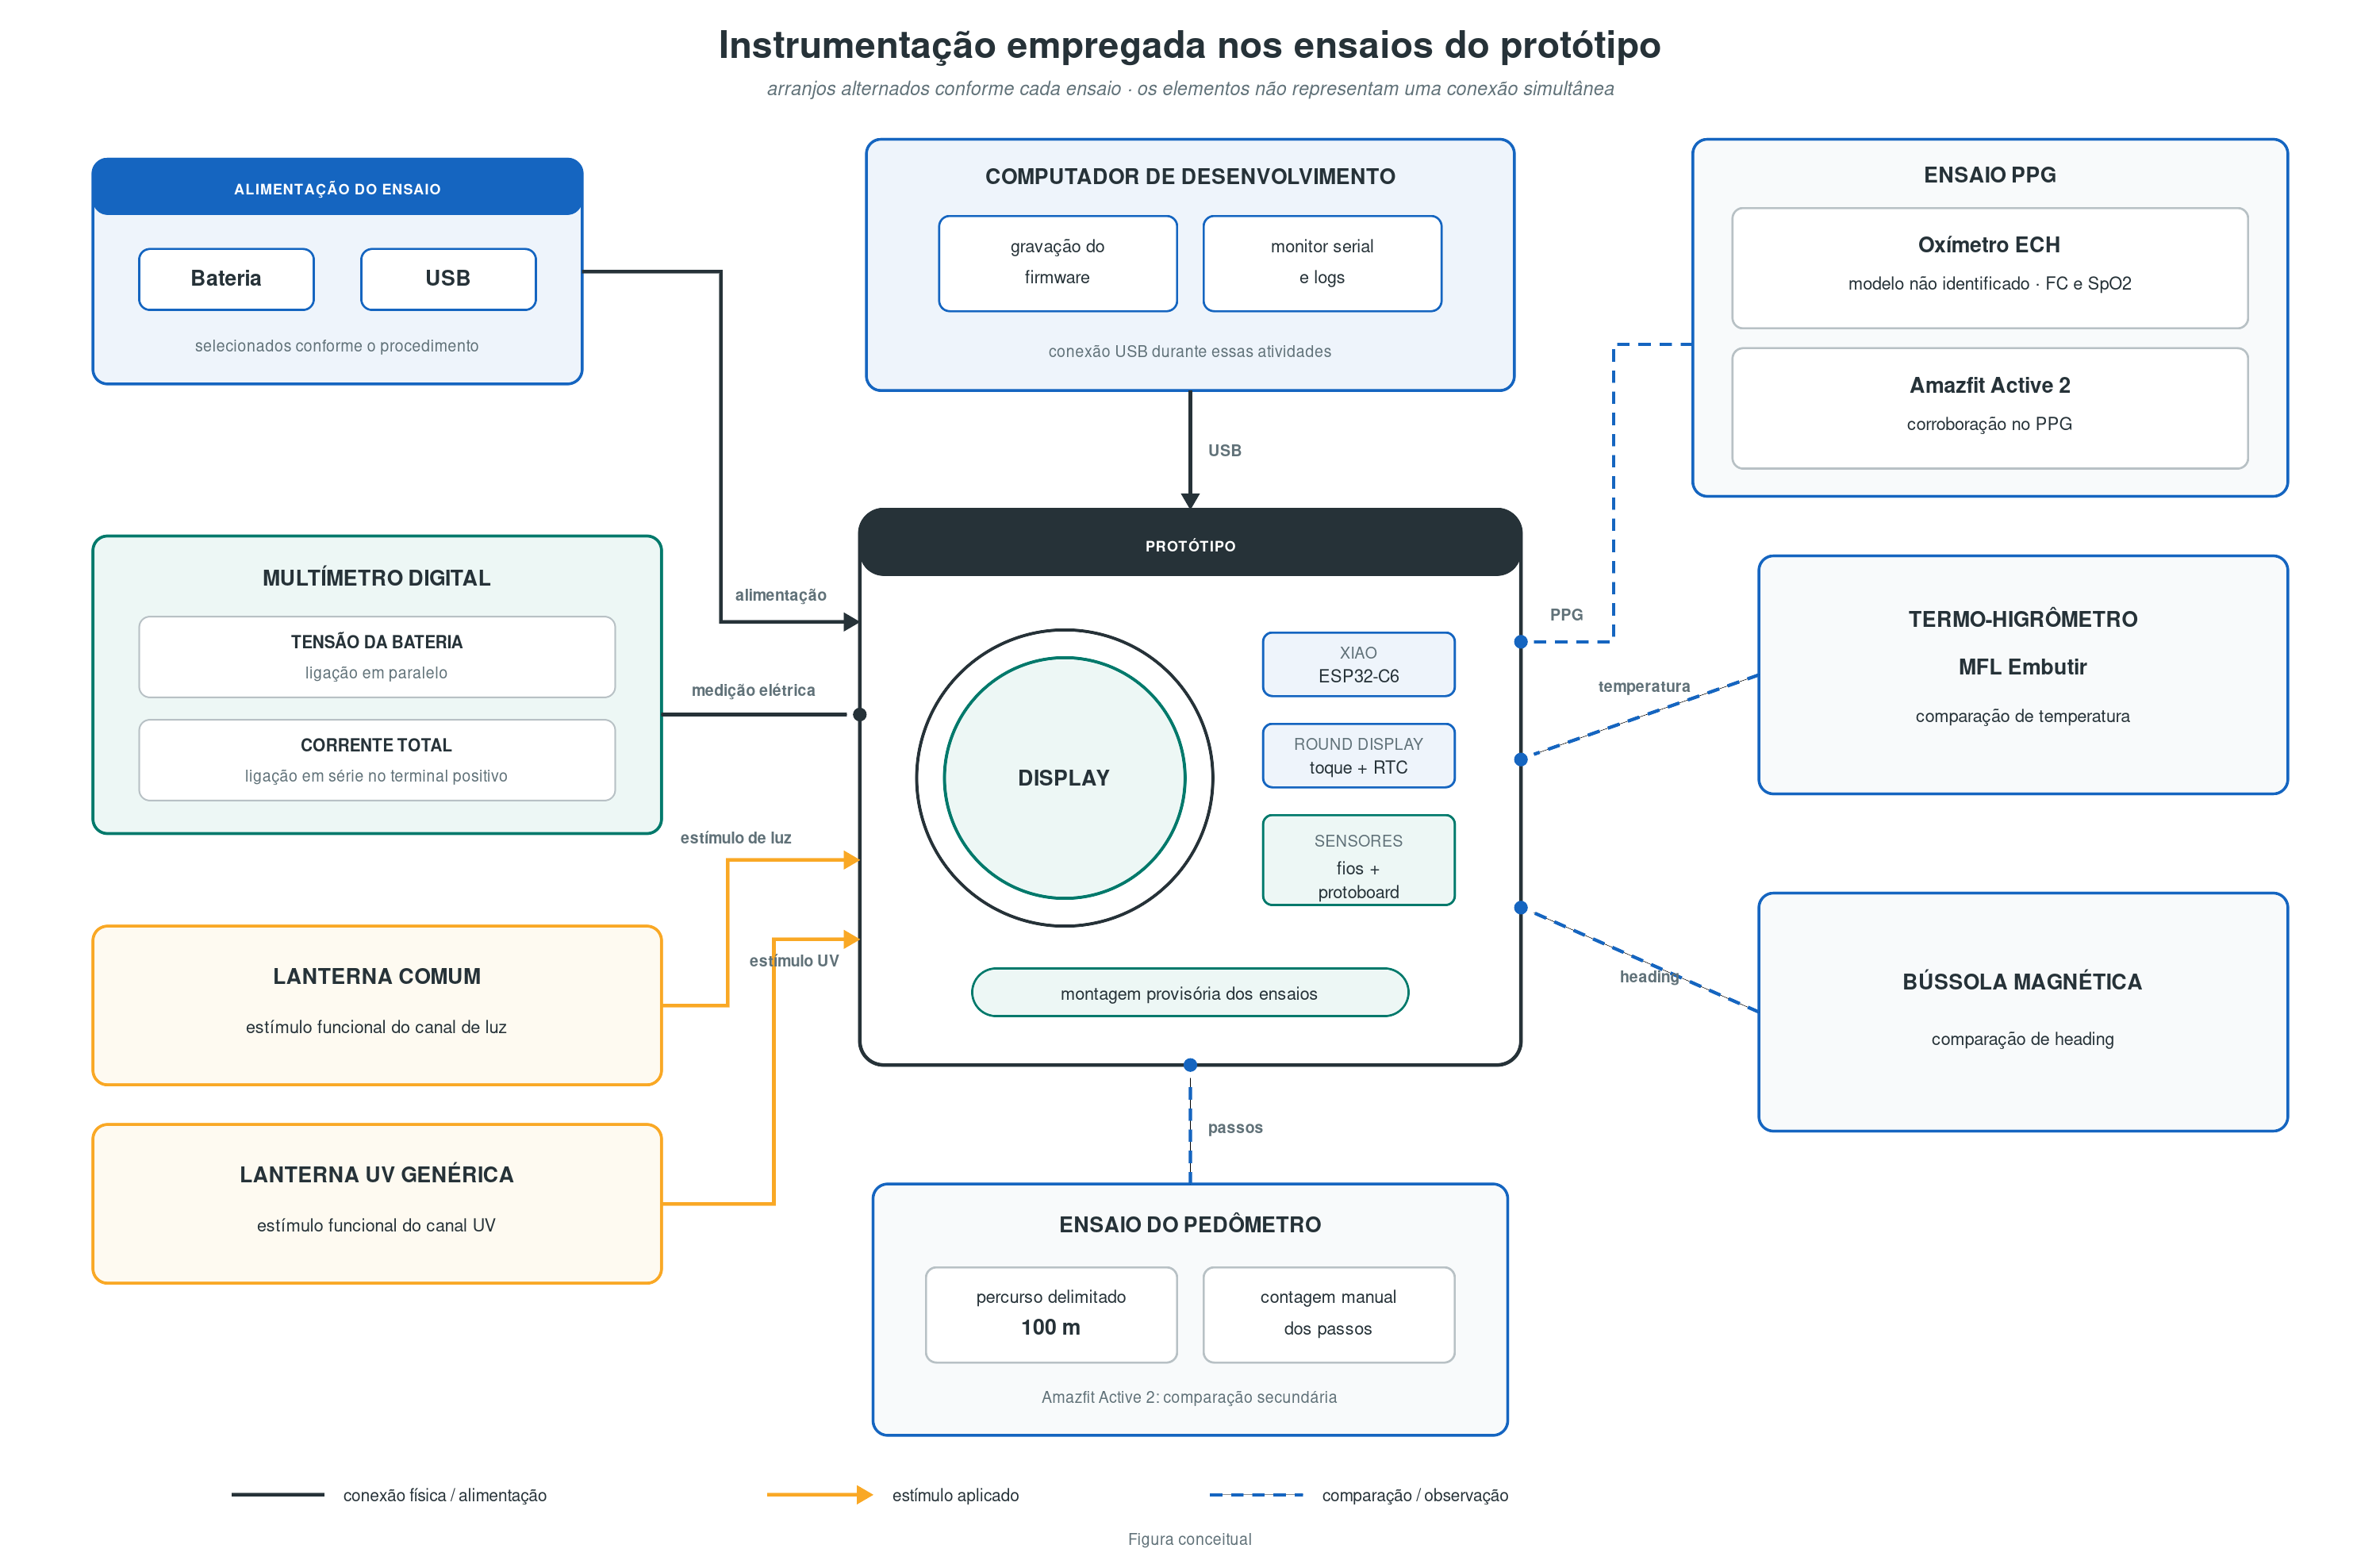
\includegraphics[width=0.96\textwidth]{Diagramas/teoricas/instrumentacao_ensaios.png}
\fonteelemento{Elaborado pelo autor a partir do caderno de ensaios}
\end{figure}


\subsubsection{Condi\c{c}\~oes comuns e rastreabilidade}


Cada coleta registrou, quando dispon\'iveis, data, local, vers\~ao do hardware, identifica\c{c}\~ao do firmware, configura\c{c}\~ao de compila\c{c}\~ao, forma de alimenta\c{c}\~ao, instrumentos, dura\c{c}\~ao e operador. Os dados brutos foram preservados em formato tabular quando houve exporta\c{c}\~ao, acompanhados do script ou procedimento usado para produzir tabelas e gr\'aficos. Lacunas desses metadados foram mantidas como limita\c{c}\~oes, sem reconstru\c{c}\~ao retrospectiva.


O n\'umero efetivo de repeti\c{c}\~oes foi informado para cada ensaio. S\'eries com uma ou duas execu\c{c}\~oes foram classificadas como pilotos ou testes funcionais limitados, e n\~ao como caracteriza\c{c}\~ao estat\'istica. Eventos inesperados, amostras descartadas e crit\'erios de exclus\~ao foram preservados no caderno de ensaios.


\subsubsection{Extensibilidade}

Como a integra\c{c}\~ao de outro componente n\~ao integrou o escopo temporal da avalia\c{c}\~ao, a extensibilidade foi examinada por estudo retrospectivo da transforma\c{c}\~ao do teste standalone do MAX30102 em m\'odulo da plataforma. Foram identificados os arquivos reutilizados, criados e modificados, as adapta\c{c}\~oes ao barramento e ao mutex compartilhados, os pontos de registro no n\'ucleo e as altera\c{c}\~oes exigidas em componentes independentes.


A an\'alise considerou o confinamento das altera\c{c}\~oes ao driver e ao m\'odulo, a quantidade de pontos de registro no n\'ucleo e a ocorr\^encia de modifica\c{c}\~oes em fun\c{c}\~oes independentes. Essa evid\^encia \'e estrutural: ela descreve o caso observado e n\~ao representa uma medida geral do tempo necess\'ario para integrar qualquer sensor.


\subsubsection{Acoplamento}


O acoplamento foi avaliado sobre a mesma vers\~ao do firmware utilizada nos demais ensaios arquiteturais. Foi constru\'ida uma matriz de depend\^encias entre n\'ucleo, servi\c{c}os, drivers e m\'odulos a partir de inclus\~oes de cabe\c{c}alhos, chamadas p\'ublicas, acesso a vari\'aveis globais e uso de recursos compartilhados.


Para cada par de componentes, foram registradas a presen\c{c}a e a dire\c{c}\~ao da depend\^encia. Chamadas realizadas por interfaces previstas no contrato foram diferenciadas de acessos diretos a dados internos ou de chamadas entre m\'odulos funcionais. A leitura conjunta do grafo e da matriz foi empregada para identificar concentra\c{c}\~oes e ciclos, sem reduzir a avalia\c{c}\~ao a uma \'unica contagem.


\subsubsection{Mem\'oria}


O uso est\'atico de mem\'oria foi obtido para uma compila\c{c}\~ao limpa do sistema integrado, por meio das ferramentas de an\'alise do ESP-IDF. Foram registrados o tamanho da imagem da aplica\c{c}\~ao e a ocupa\c{c}\~ao da parti\c{c}\~ao configurada.


N\~ao foram produzidas compila\c{c}\~oes controladas com habilita\c{c}\~ao incremental dos m\'odulos nem uma s\'erie de heap por cen\'ario. Por isso, o resultado caracteriza somente a configura\c{c}\~ao integrada e n\~ao permite atribuir um custo de mem\'oria isolado a cada m\'odulo.


\subsubsection{CPU}

A vers\~ao corrente possui um contador associado ao \emph{idle hook}, mas n\~ao foi executada uma s\'erie controlada com linha de base congelada e cen\'arios repetidos. Assim, registros explorat\'orios de ociosidade n\~ao foram empregados como medida de carga de CPU.


A caracteriza\c{c}\~ao futura dever\'a amostrar o contador em janelas fixas, estabelecer uma refer\^encia reproduz\'ivel e registrar simultaneamente heap livre e menor heap observado. Mesmo nessas condi\c{c}\~oes, o m\'etodo fornecer\'a uma estimativa global, sem separar o consumo por tarefa nem demonstrar atendimento a prazos.


\subsubsection{Tempo de boot}


Os logs de inicializa\c{c}\~ao foram usados para confirmar a sequ\^encia de cria\c{c}\~ao dos servi\c{c}os e dos m\'odulos e a continuidade do boot em condi\c{c}\~ao degradada. N\~ao foi definida uma origem f\'isica de tempo nem executada uma s\'erie repetida at\'e a disponibiliza\c{c}\~ao da interface.


Consequentemente, os registros permitem discutir ordem e toler\^ancia a falhas, mas n\~ao constituem medida de tempo de boot. Uma caracteriza\c{c}\~ao quantitativa exigir\'a evento inicial observ\'avel, crit\'erio final fixo, repeti\c{c}\~oes e resolu\c{c}\~ao temporal conhecida.


\subsubsection{Robustez do I$^2$C}


A robustez foi examinada por an\'alise est\'atica dos caminhos de erro, dos limites de espera e do mecanismo de recupera\c{c}\~ao, complementada pelos registros de integra\c{c}\~ao. O firmware serializa as transa\c{c}\~oes, propaga o erro e pode reinicializar o barramento ap\'os falha.


N\~ao foi executada uma s\'erie de falhas induzidas com medi\c{c}\~ao do tempo de recupera\c{c}\~ao e contabiliza\c{c}\~ao de sucessos. Portanto, a presen\c{c}a do mecanismo foi confirmada, mas sua efic\'acia din\^amica n\~ao foi quantificada.


\subsubsection{Sensor ausente}


Com o prot\'otipo desligado, cada sensor externo foi removido individualmente e o sistema foi religado. O procedimento tamb\'em foi repetido com sensores removidos em diversos arranjos. Em cada condi\c{c}\~ao, foram conferidos o t\'ermino da inicializa\c{c}\~ao, a tela principal, o toque, o RTC, a navega\c{c}\~ao pelos menus, a indica\c{c}\~ao de indisponibilidade da fun\c{c}\~ao dependente e o acesso aos demais m\'odulos conectados.


O ensaio teve car\'ater funcional e qualitativo: verificou se a aus\^encia de um ou mais sensores impedia o uso do restante do prot\'otipo, sem medir tempo de recupera\c{c}\~ao nem produzir uma taxa estat\'istica de disponibilidade.


\subsubsection{Ensaio prolongado}


Foi mantida uma observa\c{c}\~ao prolongada da tela principal para verificar continuidade visual e atualiza\c{c}\~ao do rel\'ogio. A dura\c{c}\~ao exata e um roteiro completo de altern\^ancia entre m\'odulos n\~ao foram preservados no registro.


Essa observa\c{c}\~ao sustenta apenas a continuidade no intervalo acompanhado. Ela n\~ao substitui um ensaio prolongado com dura\c{c}\~ao definida, navega\c{c}\~ao repet\'ivel, contadores de erro, heap e condi\c{c}\~oes ambientais registrados.


\subsubsection{MAX30102}

O ensaio funcional do MAX30102 foi executado no firmware standalone durante aproximadamente 65 s, com aquisi\c{c}\~ao a 100 Hz e sa\'ida resumida a cada segundo. Um ox\'imetro de dedo ECH e um Amazfit Active 2 foram usados simultaneamente; a an\'alise quantitativa tomou o ox\'imetro como comparador e usou o dispositivo comercial apenas como corrobora\c{c}\~ao. A configura\c{c}\~ao standalone e suas diferen\c{c}as em rela\c{c}\~ao ao firmware integrado foram registradas.


Foram registrados valores de frequ\^encia card\'iaca e SpO$_2$ ao longo de trechos temporais compar\'aveis. Os canais vermelho e infravermelho brutos foram exportados a 50 Hz, enquanto o processamento permaneceu configurado para aquisi\c{c}\~ao a 100 Hz. O transiente inicial foi separado e os sinais bruto, sem componente DC e filtrado foram produzidos por script a partir do arquivo preservado.


As leituras dos tr\^es dispositivos foram aproximadas no tempo pela observa\c{c}\~ao simult\^anea, sem rel\'ogio eletr\^onico compartilhado. A compara\c{c}\~ao foi classificada como teste funcional limitado e n\~ao como valida\c{c}\~ao cl\'inica.


\subsubsection{DS18B20}

O DS18B20 foi mantido ao lado do termo-higr\^ometro MFL Embutir durante aproximadamente 5 min em ambiente pr\'oximo de 23 $^\circ$C. Ambos permaneceram em posi\c{c}\~ao fixa; a compara\c{c}\~ao foi limitada a um ponto de opera\c{c}\~ao e classificada como verifica\c{c}\~ao de plausibilidade.


Para observar resposta transit\'oria, o prot\'otipo foi colocado em freezer com a porta fechada por 2 min, com registro ap\'os 1 e 2 min. Em ensaio separado, o probe foi aproximado da maior boca de um fog\~ao por 30 s e o aquecimento foi interrompido ao atingir 70 $^\circ$C para preservar o encapsulamento. Como n\~ao houve refer\^encia calibrada nesses transientes, o procedimento avaliou somente resposta funcional.


\subsubsection{LTR390}


Ilumin\^ancia e ultravioleta foram exercitados separadamente. Na vers\~ao integrada, cada troca de modo descarta tr\^es amostras de estabiliza\c{c}\~ao e mant\'em estados de filtragem independentes para ALS e UVS.


Para ilumin\^ancia, o sensor foi exposto a obstru\c{c}\~ao total, ambiente interno, lanterna comum, c\'eu nublado e luz solar direta. Como n\~ao havia lux\'imetro identificado, o procedimento verificou ordena\c{c}\~ao qualitativa da resposta e ocorr\^encia de satura\c{c}\~ao, sem validar quantitativamente a unidade lux.


Para UVI, a leitura externa foi comparada com uma refer\^encia meteorol\'ogica correspondente ao local e ao dia. Essa fonte n\~ao equivalia a um radi\^ometro colocado junto ao prot\'otipo e foi usada somente como contexto de plausibilidade.

Em teste standalone adicional, uma lanterna UV gen\'erica foi aproximada de cerca de 20 cm at\'e muito pr\'oximo do sensor. Esse procedimento avaliou somente se a indica\c{c}\~ao aumentava com a aproxima\c{c}\~ao da fonte, pois seu espectro e irradi\^ancia n\~ao eram conhecidos.


\subsubsection{B\'ussola}

Antes da coleta, a calibra\c{c}\~ao em 12 setores foi executada no pr\'oprio dispositivo. O prot\'otipo e a b\'ussola Norvix DC45-2 foram mantidos no mesmo plano horizontal, sem ajuste de declina\c{c}\~ao. Foram comparadas duas orienta\c{c}\~oes separadas por aproximadamente meia-volta.


A diferen\c{c}a foi calculada diretamente entre as indica\c{c}\~oes magn\'eticas. Como foram avaliadas apenas duas orienta\c{c}\~oes e a refer\^encia n\~ao era calibrada, o ensaio foi tratado como teste funcional de resposta direcional, sem alega\c{c}\~ao de precis\~ao.


\subsubsection{Ped\^ometro}

O ensaio controlado utilizou um percurso de 100 m delimitado pela ferramenta de medi\c{c}\~ao do Google Maps. Um participante percorreu o trecho na ida e na volta em ritmo habitual, com o prot\'otipo e o Amazfit Active 2 no pulso. Os passos foram contados manualmente e adotados como refer\^encia.


Para cada percurso foram registrados passos de refer\^encia, passos detectados pelo prot\'otipo e passos informados pelo dispositivo comercial. Foram calculados erro absoluto e erro relativo. O ensaio foi limitado a um participante, um ritmo e duas repeti\c{c}\~oes.


\[
E_{\mathrm{abs}}=N_{\mathrm{detectado}}-N_{\mathrm{referencia}},
\qquad
E_{\mathrm{rel}}=\frac{|E_{\mathrm{abs}}|}{N_{\mathrm{referencia}}}\times 100\%.
\]


O contador foi reiniciado antes de cada repeti\c{c}\~ao, pois sua persist\^encia n\~ao faz parte da implementa\c{c}\~ao. Os resultados foram limitados \`as condi\c{c}\~oes e ao posicionamento ensaiados.


\subsubsection{Bateria}

A tens\~ao indicada pelo ADC foi comparada com o mult\'imetro nas condi\c{c}\~oes com USB e somente com bateria. Em ensaio separado, o mult\'imetro foi ligado em s\'erie com o terminal positivo da bateria e a corrente foi observada em nove cen\'arios funcionais ap\'os intervalo de estabiliza\c{c}\~ao.

N\~ao foi executada curva de descarga completa. A autonomia foi apenas estimada pela raz\~ao entre uma capacidade \`util assumida de aproximadamente 1000 mAh e as correntes observadas. Esses valores n\~ao foram apresentados como autonomia medida, e as proje\c{c}\~oes com modos de baixo consumo foram reservadas aos trabalhos futuros.

\end{document}
